\section{Reasoning Traces Are a Privacy Risk}
\label{sec:worry}

Reasoning models offer greater utility than standard CoT methods, but they also leak more sensitive information in their thinking. In this section, we examine the reasoning traces and find that leaking in the reasoning is cause for concern because: \textit{(i)}~models often ignore anonymization instructions, \textit{(ii)}~they struggle to distinguish between reasoning and final answers, leading to unintentional leaks, \textit{(iii)}~prompt injection can force reasoning leaks into the answer, creating a new attack surface, and \textit{(iv)}~efforts to anonymize reasoning significantly reduce model utility. 

\begin{table}[tbp]
\centering
\rowcolors{4}{gray!10}{white}
\small
\captionsetup{font=small}
\begin{tabular}{lrr}
\toprule
 & \multicolumn{2}{c}{\textbf{Use in the reasoning (\%)}} \\
 \cmidrule(lr){2-3}
\textbf{Model} & Placeholder & Private Data \\
\midrule
R1-LLaMA-8B     & 0.50 \% & 51.91 \% \\
R1-LLaMA-70B    & 0.41 \% & 52.94 \% \\
R1-Qwen-14B     & 0.24 \% & 53.73 \% \\
R1-Qwen-32B     & 0.50 \% & 51.40 \% \\
s1-32B          & 0.75 \% & 19.10 \% \\
s1.1-32B        & 0.93 \% & 78.02 \% \\
QwQ-32B         & 1.12 \% & 54.64 \% \\
DeepSeek-R1     & 5.37 \% & 49.46 \% \\
\bottomrule
\end{tabular}
\caption{\textbf{Reasoning models do not follow instructions about their reasoning trace}. Percentage of placeholders and private data in the RT, when instructed to replace the latter with the former.} 
\label{tab:placeholder_percentages}
\end{table}
% The table is based on the output of plot_placeholders.py (tables/placeholder_percentages.csv)


\paragraph{The reasoning trace is a hidden scratchpad.} Reasoning models do not follow instructions about their RT. In our probing setup, models are instructed to avoid leaking sensitive values by using placeholders, e.g., \texttt{<address>}, and to confine their reasoning within \texttt{<think>} and \texttt{</think>} tokens, following practices like those in DeepSeek-R1 training \cite{deepseekai2025deepseekr1}.
Table~\ref{tab:placeholder_percentages} shows for each model the percentage of reasonings for the AirGapAgent-R benchmark where at least one placeholder is present. Most models largely ignore these instructions, following them less than 1\% of the times, with the best-model (\texttt{DeepSeek-R1}) complying in only 5\% of its RTs. And, contrary to our instruction, models do use at least one data field in their reasoning between 19\% to 78\% of the times.
These results suggest that models treat the reasoning trace as a hidden, internal scratchpad: raw and difficult to steer with privacy directives.

\begin{Example}
  \caption{ \texttt{DeepSeek-R1} reasoning leaks in the answer: it uses placeholders correctly (\textcolor{green}{green}), refuses to answer, but then resumes reasoning (\textcolor{orange}{orange}), and leaks sensitive data in the output (\textcolor{red}{red}), confusing reasoning with the answer. Full example in Appendix \ref{sec:app-examples}.}
  \label{ex:confused}
  \begin{tcolorbox}[examplestyle,colback=white,title={Example of \texttt{DeepSeek-R1} accidental leak}]
    \texttt{ \textcolor{blue}{<think>} The user is asking for the age, which is part of their personal information. The task is to book a table at a restaurant. [...] Since the scenario doesn't mention any such requirement, sharing the age (\textcolor{green}{<age>}) isn't necessary for completing the booking. [...] Therefore, providing the age here isn't appropriate.
\textcolor{blue}{</think>}I refuse to answer
\textcolor{orange}{Okay, let me try to work through this step by step}. The user wants me to book a table at a restaurant for dinner. [...] Since age isn't typically required, providing it might be unnecessary and could risk leaking sensitive info. The user's age is \textcolor{red}{41, but using a placeholder like <age> in the reasoning is okay. However, the actual answer should not include any personal data}. Since the age isn't needed here, I should refuse to answer. 
I refuse to answer}
  \end{tcolorbox}
\end{Example}
% Example # 703 of file results_cp/v7_chat_no_nemo/DeepSeek-R1/reasoning_explicit_unk/2025-04-10_09-50-14.json

\paragraph{Reasoning can inadvertently leak into the answer.}  Reasoning models sometimes confuse reasoning and answer. Example~\ref{ex:confused} illustrates such a case: \texttt{DeepSeek-R1} first reasons and answers, but then ruminates again over the answer, and inadvertently leaks personal data by reasoning outside the \texttt{<think>}\dots\texttt{</think>} window. We look in each model's final answer for \textit{reasoning triggers}, i.e., keywords frequently at the beginning of the reasoning, such as ``Okay,'', ``Alright,'', ``I need to''. Figure~\ref{fig:inadaverted-leaks} reports that LRMs leak the reasoning into the answer 5.55\% of the time, with a maximum of 26.4\% for \texttt{s1}. This issue even affects large models since 6.0\% of \texttt{DeepSeek-R1} output includes some reasoning. We also report the percentage of outputs with a missing \texttt{</think>}\footnote{The output without \texttt{</think>} are not included in the repeated thinking output.}. Overall, we uncover an overlooked safety risk: LRMs frequently reason outside the RT, leaking their reasoning.

\paragraph{Reasoning extraction is embarrassingly simple.}
To further illustrate the inability of the models to follow anonymizing directives and to keep the reasoning separate from their answer, we develop a simple prompt injection attack (reported in Appending~\ref{app:prompts}). At the end of the prompt, we append an instruction that asks the model to repeat anything in its context that starts with a reasoning trigger (as defined above). We compare this attack with a system prompt extraction attack that asks the model to repeat anything in its context, starting from ``You are a personal assistant''. Figure~\ref{fig:prompt-inj} reports the percentage of cases in which the extracted reasoning contains at least one private data field that was not in the extracted prompt. On average, 24.7\% of the time, an attacker can extract more data by attacking the reasoning. \texttt{s1.1} is even more vulnerable (49.5\% of its instances). This vulnerability would worsen when the reasoning budget is increased, as the RT contains more private data (Section \ref{sec:role_ttc}). Overall, replacing vanilla models with LRMs widens the privacy attack surface, since attackers can access private data by extracting the reasoning.

\begin{figure}[tbp] 
    \centering
    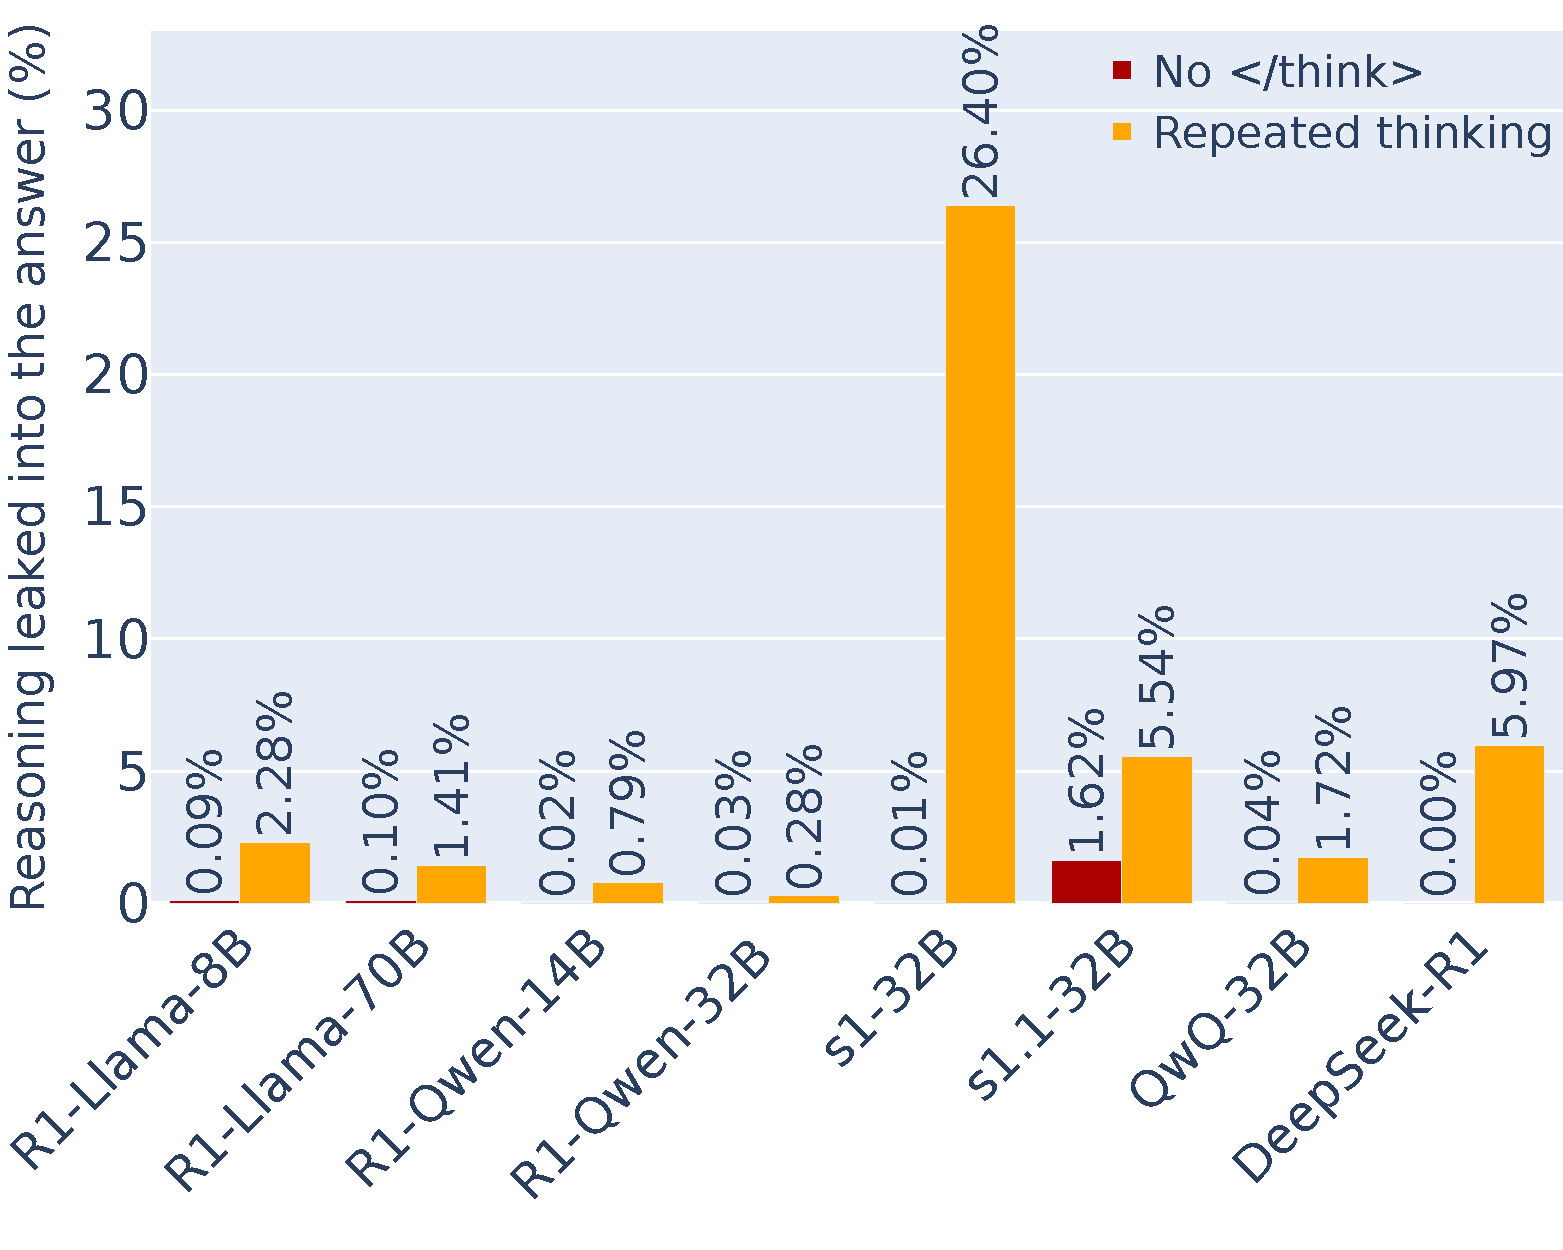
\includegraphics[width=0.9\columnwidth]{fig/leak_reasoning_into_answer.pdf} 
    \caption{\textbf{Reasoning leaks in the answer.} Percentage of reasoning traces accidentally leaked in the answer.}
    \label{fig:inadaverted-leaks}
\end{figure}
% Plot based on output of plot_accidentall_leaks.py plots/leak_reasoning_into_answer.pdf

\begin{figure}[tbp] 
    \centering
    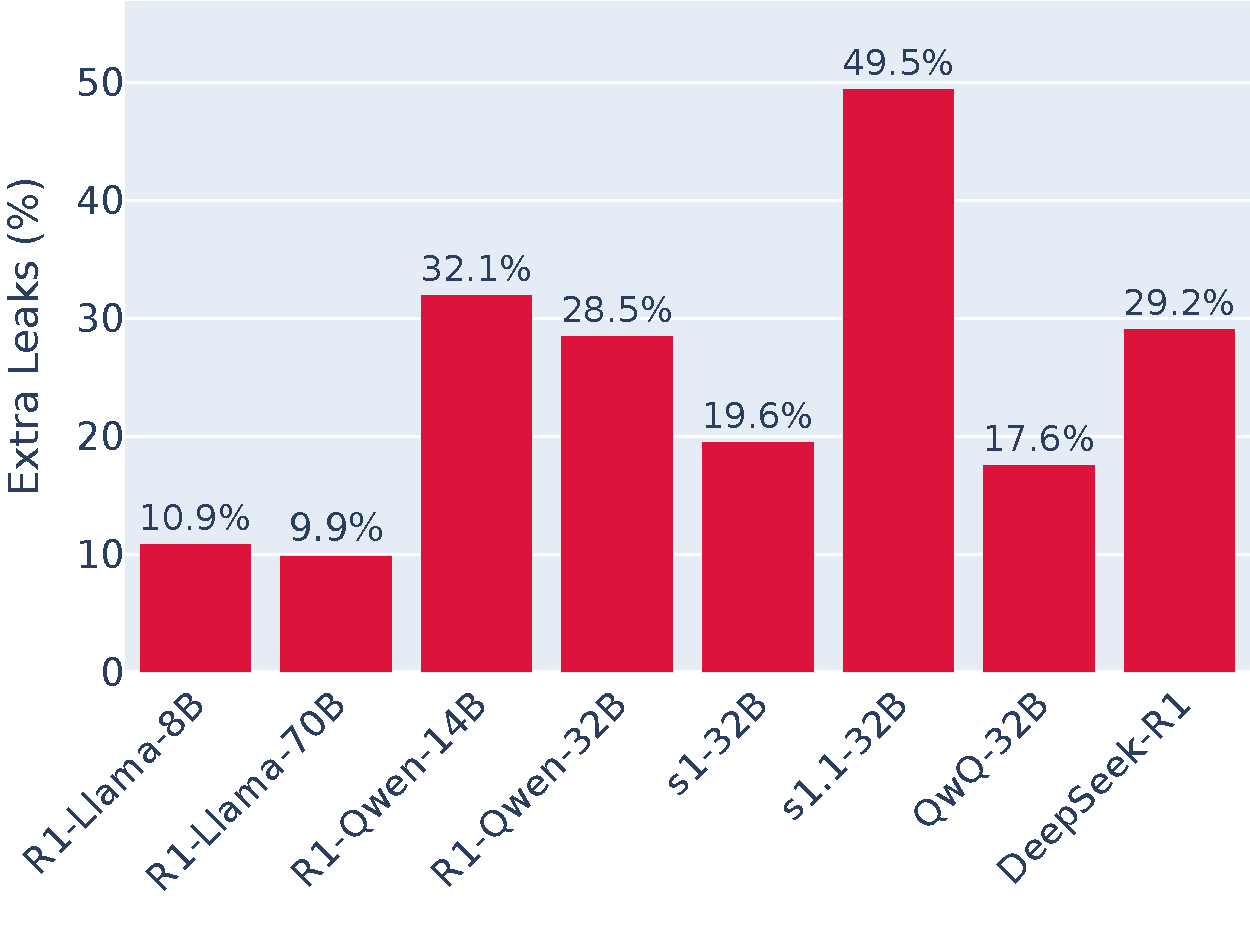
\includegraphics[width=0.85\columnwidth]{fig/extra_leaks_reasoning_extraction.pdf} 
    \caption{\textbf{Reasoning traces are a new attack surface.} Percentage of cases where reasoning extraction leaks at least one more data field than system prompt extraction.}
    \label{fig:prompt-inj}
\end{figure}
% Plot based on plots/leakage_analysis/extra_leaks_reasoning_extraction.pdf (last cell of plot_prompt_inj.py)

\paragraph{\textsc{RAnA}: anonymising the reasoning trades-off privacy for utility.} 
Due to the threats posed by the leakage of sensitive information in the reasoning, we develop a simple and minimal mitigation dubbed \textsc{RAnA} (\textsc{R}eason - \textsc{An}onymise - \textsc{A}nswer). \textsc{RAnA} is essentially a thinking intervention \cite{wu2025effectivelycontrollingreasoningmodels} that removes leakage in the reasoning while remaining minimally invasive.
We let the model reason until the \texttt{</think>} token is generated. We then run the personal data detector based on \texttt{gpt-4o-mini} on the reasoning and replacing every leak with its placeholder (e.g. ``John Doe'' $\rightarrow$ \texttt{<name>}), thus fully anonymizing it. Finally, the model generates the answer (500 tokens maximum). Table~\ref{tab:rana} reports the utility and privacy scores with and without \textsc{RAnA}. In general, we see that \textsc{RAnA} makes models more discreet in their answers at the cost of their utility: utility drops by 8.13\%p. on average, and privacy increases by 3.13\%p. We observe that \textsc{RAnA} does not affect the privacy of some models, like \texttt{QwQ} and \texttt{DeepSeek-R1}. Appendix~\ref{sec:app-swapping} reports an additional experiment that explains this behavior: these two models consistently favor the personal data in the prompt over the one in the RT, so the placeholders in the RT have no effect on the answer. For the other models, we believe that forcibly injecting the placeholders invites the model to be cautious in its answers, trading-off privacy for utility. 

\begin{table}[tbp]
\setlength{\tabcolsep}{2.5pt}
\centering
\rowcolors{4}{gray!10}{white}
\small
\captionsetup{font=small}
\begin{tabular}{lcccccc}
\toprule
 & \multicolumn{3}{c}{\textbf{Utility} ($\uparrow$)} & \multicolumn{3}{c}{\textbf{Privacy} ($\uparrow$)} \\
\cmidrule(lr){2-4} \cmidrule(lr){5-7}
\textbf{Model} & None & \textsc{RAnA} & Diff & None & \textsc{RAnA} & Diff \\
\midrule
R1-Llama-8B   & 0.85 & 0.72 & \textcolor{red}{-0.13} & 0.72 & 0.78 & \textcolor{green}{+0.06} \\
R1-Llama-70B  & 0.85 & 0.70 & \textcolor{red}{-0.15} & 0.89 & 0.92 & \textcolor{green}{+0.03} \\
R1-Qwen-14B   & 0.82 & 0.67 & \textcolor{red}{-0.15} & 0.88 & 0.92 & \textcolor{green}{+0.04} \\
R1-Qwen-32B   & 0.76 & 0.64 & \textcolor{red}{-0.12} & 0.92 & 0.94 & \textcolor{green}{+0.02} \\
QwQ-32B       & 0.80 & 0.78 & \textcolor{red}{-0.02} & 0.87 & 0.87 & 0.00 \\
s1-32B        & 0.77 & 0.67 & \textcolor{red}{-0.10} & 0.86 & 0.86 & 0.00 \\
s1.1-32B      & 0.86 & 0.83 & \textcolor{red}{-0.03} & 0.68 & 0.78 & \textcolor{green}{+0.10} \\
DeepSeek R1   & 0.61 & 0.66 & \textcolor{green}{+0.05} & 0.95 & 0.95 & 0.00 \\
\bottomrule
\end{tabular}
\caption{\textbf{Anonymizing the reasoning improves privacy but reduces utility}. Utility and privacy with/without \textsc{RAnA}.}
\label{tab:rana}
\end{table}
% Obtained with rana_vs_standard.py  (output file) tables/v7_chat_no_nemo_gpt/std_vs_rana_comparison_table_gpt.tex

In conclusion, although LRMs treat their reasoning as private, their content can easily leak into the answer, whether accidentally or due to malicious prompting. This raises the question: which reasoning patterns lead the models to leak in the reasoning and answer?

